\chapter{The CMS detector and the Large Hadron Collider}
\label{c:det}
This chapter discusses the Large Hadron Collider (LHC) which is located on the Franco-Swiss border near Geneva approximately 100 m undergrounds at the site of the Centre European de Research Nuclear (CERN). It is a 26.7 km long synchrotron particle accelerator with four interaction points where four experiments are located.  My thesis focuses on results from the Compact Muon Solenoid detector described in section~\ref{sec:CMSdet}. The other experiments include ATLAS which is a multi-purpose experiment like CMS, the LHCb detector which focusses on the study of the physics of B mesons and the ALICE detector which is used to study quark-gluon plasmas.

\section{LHC}

The LHC accelerates two beams of protons which circulate in opposite directions \fixme{describe opposite magnetic dipoles}. The protons are sourced from a bottle of hydrogen where a strong electric field is used to rip apart the electrons from the hydrogen atom leaving protons behind. The protons are then accelerated through the linear accelerator LINAC2 before being injected into the Proton Synchrotron Booster (PSB), then into the Proton Synchrotron (PS) followed by the Super Proton Synchrotron (SPS) which is the final accelerator before the protons are injected into the LHC ring. Each accelerator stage boosts the protons to a higher energy, as seen in fig.\fixme{add figure} before they can be injected into the LHC where their final collision energy can be achieved.

\begin{figure}[ht!]
\centering
    \includegraphics[width=0.95\textwidth]{images/LHCacc.jpg}
    \caption{The LHC accelerator complex at CERN}
    \label{fig:LHC acc}
\end{figure}


 The LHC was designed to have a centre of mass collision energy of $\sqrt{s} = 14 \TeV$. However, after an incident 10 days into operation in 2008 which caused damage to the LHC, it was restarted with the lower energy of $\sqrt{s} = 7 \TeV$ in 2011. In 2012 this was increased to $\sqrt{s} = 8 \TeV$ and a dataset with a \fixme*{explain lumi}{luminosity} of $\approx 20 \fbinv$ was recorded. This dataset was used for the analysis in chapter~\ref{c:Run1}. Further details on the run conditions can be found in \fixme{table of lumi, bunches etc.}. In 2013 after the run phase known as \emph{Run 1}, Long Shutdown 1 (LS1) commenced to make upgrades to the LHC and the detectors to allow the machine to run at $\sqrt{s} = 13 \TeV$ for \emph{Run 2}. Run 2 began in March 2015 and results from Run2 are the focus of the analysis in chapter~\ref{c:Run2}.

Run1 saw the great success of the discovery of the Higgs boson, one of the main objectives of the LHC. In Run2, the search for new physics continues where precision measurements will test the predictions of the Standard Model.

\section{CMS detector \label{sec:CMSdet}
}

\begin{figure}[ht!]
\centering
    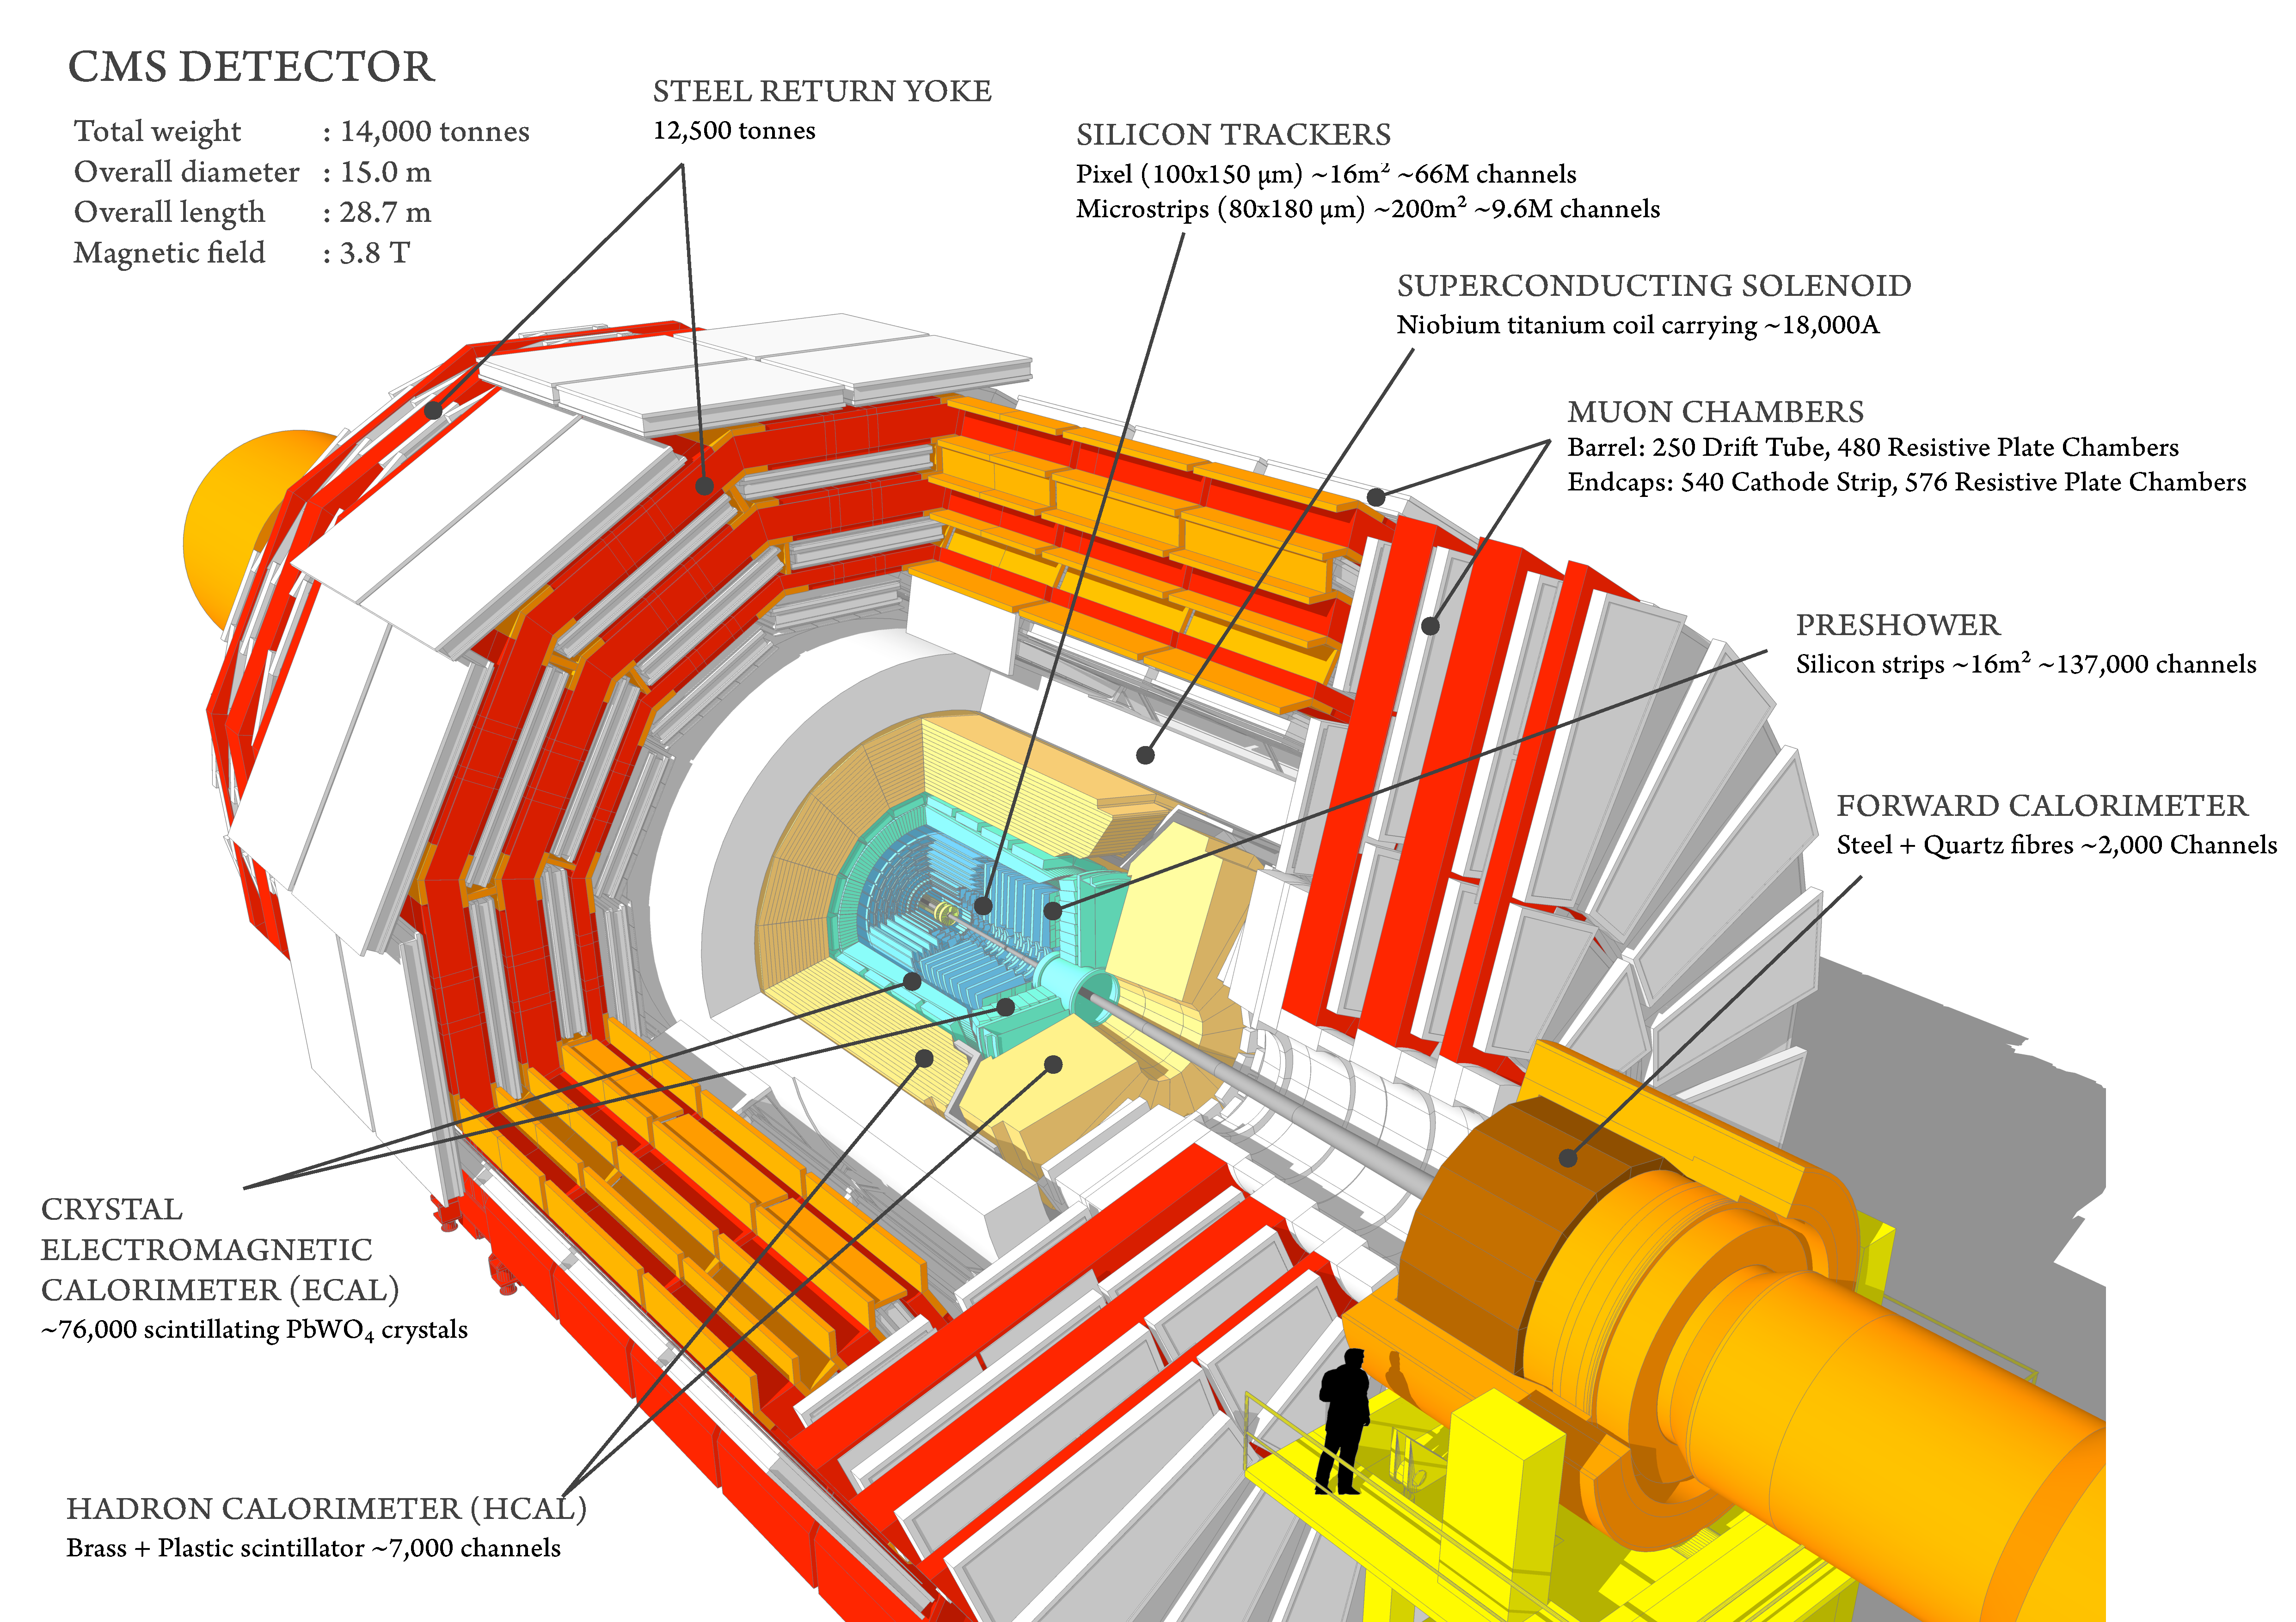
\includegraphics[width=0.95\textwidth]{images/cmsdetector3.pdf}
    \caption{The CMS detector~\cite{1742-6596-513-2-022032}}
    \label{fig:CMSdetector}
\end{figure}

\subsection{Magnetic Solenoid}

The superconducting magnetic solenoid at the core of CMS was designed to have a magnetic field of 4 T. The free bore magnet has a diameter of 6.3 m and length of 12.5 m. It uses 4-layer winding of NbTi conductor which is required to generate this high magnetic field. The magnet is cooled within a cryostat to a temperature of 4.5K using liquid helium. The magnetic field is returned via an iron yoke consisting of five barrel wheels and two endcaps which are made of three discs each. The outer dimension of the iron flats is 14 m.
The solenoid provides a homogeneous magnetic field over the tracking region which bends particle trajectories transverse to the beam direction.
% described in section~\ref{sec:tracker}

\subsection{Tracker \label{sec:tracker}}

The tracking system of CMS lies inside the superconducting solenoid and surrounds the interaction point. It is 5.8 m long with a diameter of 2.5 m.
Silicon detectors were used as they can provide the high granulity and fast response required to reliably reconstruct the trajectories of particles coming from the collision vertex.
% and from the secondary vertices which originate from decaying particles. 
Reconstructing secondary vertices is also particularly important for identifying jets originating from heavy flavour quarks such as bottom quarks. This is integral for distinguishing final states involving top quarks. Silicon detectors also have the radiation hardness to last for the design time of ten years. The minimum material possible was used in order to reduce the amount of multiple scattering, photon conversion and bremsstrahlung. However the high density of electronics mean that the tracker requires cooling to zero degrees celcius in Run 1 and -20 degrees celcius in Run2. Cooling also helps prevent `thermal runaway' from leakage current. 
\fixme{1000 particles 20 PU - overlapping p-p collisions}
%good to limit interaction with material in tracker

The tracking system consists of two main sections; the pixel tracker makes up the innermost section and the strip tracker surrounds the pixel tracker as seen in Fig.~\ref{fig:CMSdetector}. Tracking information is used in the high level trigger (HLT)


\begin{figure}[ht!]
\centering
    \includegraphics[width=0.95\textwidth]{images/TrackerWhole.png}
    \caption{The tracking system in Run 1~\cite{1748-0221-3-08-S08004}}
    \label{fig:TrackerWhole}
\end{figure}

\textbf{Pixel tracker}\\

As the pixel detector is closest to the interaction vertex, it experiences the highest fluence of particles at $\approx$ 1 MHz per mm$^{2}$. The fine granularity of the pixel detector (100 x 150 $\mu$ m in r-$\phi$ x z) is required in order to keep the occupancy below 1\%. It consists of three barrel layers which range between 4cm and 10.2cm from the interaction point and 2 disks which are transverse to be beamlines as seen in Fig.~\ref{fig:TrackerWhole} and Fig.~\ref{fig:pixel}.\\

\textbf{Strip tracker}\\
Two types of silicon strip tracker are used. Closest to the interaction point (20 - 50 cm) are the tracker inner barrel detectors (TIB) which contain silicon micro-strips (10cm x 80 $\mu$m). An occupancy of $\approx$ 2 - 3~\% is achieved for a fluence of $\approx$ 60 kHz per mm$^{2}$.
An increased strip pitch of 180$\mu$m can be used in the tracker outer barrel (TOB) due to the lower fluence of 3 kHz per mm$^{2}$. To cover the larger surface area the strip length is increased to 25 cm. However increased strip length increases the noise. To combat this the strips are made thicker to 500 $\mu$m compared to 320$\mu$m in the TIB.
\fixme{TEC and TID}
\fixme{Mention doping?}
\fixme{Depletion voltage?}

\subsection{Electromagnetic Calorimeter}

\subsection{Hadronic Calorimeter}

\subsection{Muon Chambers}

\subsection{Trigger}



\subsection{Upgrades for Run II}



\begin{figure}[ht!]
\centering
    \includegraphics[width=0.55\textwidth]{images/TrackerUpgradeXSec.png}
     \includegraphics[width=0.42\textwidth]{images/TrackerUpgradeBarrel.png}          
    \caption{Pixel tracker with half initial and half upgrade geometries~\cite{1742-6596-513-2-022032}}
    \label{fig:pixel}
\end{figure}


